\subsection{Overview of Drone-Based Landmine Detection Techniques}\label{sensor_overview}

Landmine detection technologies have evolved to encompass a wide range of sensing principles, each targeting specific physical, chemical, or biological characteristics of surface-laid and buried mines. 

Landmine detection relies on a variety of sensing techniques, each designed to identify specific physical, chemical, or biological features of buried or surface-laid explosives. These methods can be grouped into five main categories: \textbf{electromagnetic induction-based} techniques, \textbf{radiowave and microwave-based} systems, \textbf{spectral and thermal imaging} approaches, \textbf{mechanical and vibro-acoustic} methods, and \textbf{chemical and biological} sensing methods. Within each class, a variety of specialized technologies have been developed, including metal detectors, \gls{GPR}, optical and infrared cameras, seismic/acoustic sensors, biosensors, etc. Each approaches offers distinct advantages and faces unique limitations, especially when adapted to \gls{UAV} platforms for remote and efficient minefield scanning. In the following subsections, each class is reviewed in details focusing on their working principles and drone applications.



\subsubsection{Electromagnetic Induction-Based Techniques}\label{EMI}

\gls{EMI} methods operate by exploiting the interaction between electromagnetic fields and conductive or magnetic materials in the ground. These systems are typically composed of a transmitter coil that emits a time-varying electromagnetic field into the soil. When this field encounters a conductive object, such as a landmine with metallic components, it induces eddy currents within the object, which in turn generate a secondary magnetic field. This field is detected by a receiver coil, and the resulting signal is processed to infer the presence of the object. These principles form the basis of conventional \textbf{metal detectors}~\cite{gichd2006guidebook}.

In contrast, \textbf{magnetic sensors} or magnetometers do not actively induce eddy currents but instead measure disturbances in the Earth's ambient magnetic field caused by nearby ferromagnetic objects. While metal detectors rely on electromagnetic induction to detect a wide range of conductive materials, magnetometers are primarily sensitive to ferrous (iron-containing) materials and are particularly effective in detecting anomalies in the magnetic environment\footnote{\url{https://www.sphengineering.com/integrated-systems/technologies/magnetometer}}.

Several specialized \gls{EMI} sensors have been developed, including induction coil imaging systems that generate spatial maps of subsurface metallic objects, conductivity meters that monitor variations in soil conductivity through eddy current decay, and a range of magnetometers such as fluxgate, proton precession, optically pumped atomic, and meandering winding designs. Each sensor type offers specific trade-offs in sensitivity, resolution, and robustness, and may be selected based on the expected mine characteristics and deployment constraints~\cite{Gooneratne2004ARO, Bruschini1997ASO}.

\paragraph{Drone Applications} \gls{EMI}-based sensors have been applied to \gls{UAV} platforms in a number of recent studies~\cite{yoo2020drone,yoo2021application,rs16162916,Yoo2024UnmannedAV}. These implementations include both metal detectors and magnetometers mounted on drones for low-altitude scanning of mine-affected areas. Figure~\ref{fig:metal_detector_drone} shows an example of a \gls{UAV} equipped with a metal detector, while Figure~\ref{fig:magnetometer_drone} illustrates a drone-mounted magnetometer system. Among these approaches, \textbf{magnetometers} have emerged as the most commonly used \gls{EMI} technique in \gls{UAV}-based landmine detection research.

Despite their low cost and light weight, magnetometer-based \gls{UAV} systems face several significant limitations that hinder their effectiveness in practical demining scenarios. First, effective detection of small metallic objects typically requires low flight altitudes (often below 1 meter) to maintain a strong magnetic signal-to-noise ratio~\cite{yoo2020drone,Yoo2024UnmannedAV}. This constraint increases the risk of collision with obstacles and complicates \gls{UAV} control, particularly in rugged or vegetated terrain. Second, magnetometers are highly susceptible to electromagnetic interference generated by the drone’s motors, battery cables, and onboard electronics. To mitigate this, the sensors must be physically separated from the \gls{UAV} by a distance of 1--2 meters~\cite{Yoo2024UnmannedAV,rs16162916}. While this approach reduces magnetic noise, it also introduces mechanical complexity and reduces system stability, especially during low-altitude flight in cluttered environments. Most importantly, magnetometers are fundamentally limited in their detection scope: they are ineffective against plastic or low-metal-content landmines~\cite{garcia2020airborne,vsipovs2020lightweight}.

\begin{figure}[h!]
    \centering
    \begin{subfigure}[b]{0.48\linewidth}
        \centering
        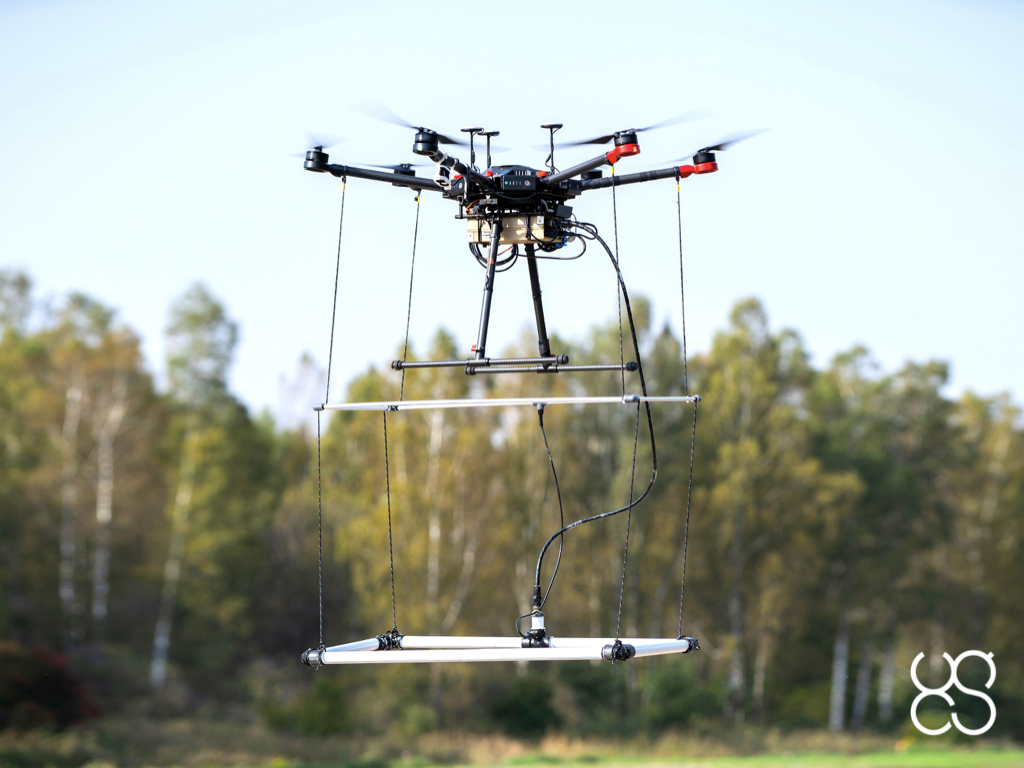
\includegraphics[height=5cm]{figs/Huirui/metal_detector_drone.png}
        \caption{UAV-mounted metal detector system\protect\footnotemark.}
        \label{fig:metal_detector_drone}
    \end{subfigure}
    \hfill
    \begin{subfigure}[b]{0.48\linewidth}
        \centering
        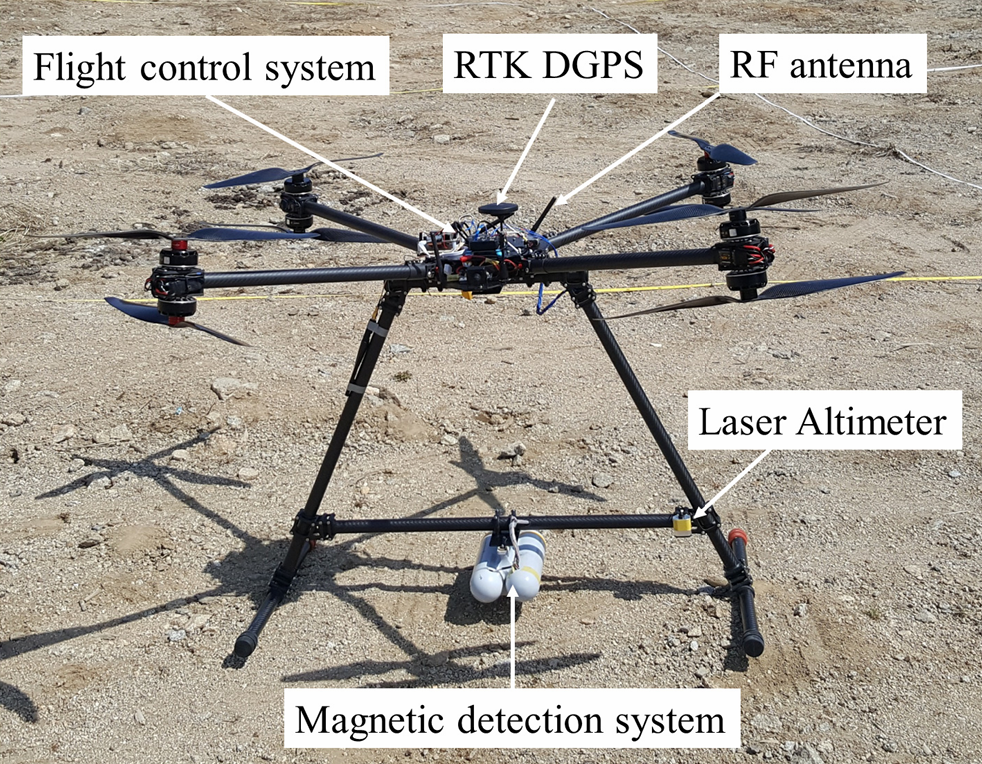
\includegraphics[height=5cm]{figs/Huirui/magnetometer_drone.png}
        \caption{Drone-based magnetometer platform~\cite{yoo2020drone}.}
        \label{fig:magnetometer_drone}
    \end{subfigure}
    \caption{Examples of UAV platforms integrating electromagnetic sensors for landmine detection.}
    \label{fig:emi_uav_examples}
\end{figure}

\footnotetext{\url{https://www.sphengineering.com/news/sph-engineering-introduces-the-drone-integrated-metal-detection-system}}



\subsubsection{Radiowave and Microwave-Based Systems}\label{Radiowave}

\gls{GPR} is a non-invasive geophysical technique that uses electromagnetic waves in the microwave frequency range (typically from several hundred MHz to a few GHz) to detect subsurface anomalies~\cite{gichd2006guidebook}. Unlike \gls{EMI}-based systems, which respond to conductive or magnetic properties, \gls{GPR} is sensitive to variations in the dielectric properties of materials~\cite{Gooneratne2004ARO}. It operates by transmitting short-duration radio pulses into the ground via a wideband antenna. When these pulses encounter boundaries between materials with different dielectric constants—such as between soil and a buried landmine—they are partially reflected. The reflected signals are then captured by a receiving antenna, and the time delay and intensity are analyzed to estimate the depth, shape, and dielectric contrast of subsurface targets~\cite{alqudsi2021review,paik2002image}.

As the antenna is moved across the ground, successive measurements are combined to construct two-dimensional slices (radargrams) or even three-dimensional volumetric representations of the subsurface~\cite{Bruschini1997ASO}. The effectiveness of \gls{GPR} depends heavily on the contrast between the dielectric properties of the object and the surrounding soil. High-frequency systems offer better resolution and are more suited for detecting small anti-personnel mines, while lower-frequency systems provide deeper penetration but at the cost of detail~\cite{gichd2006guidebook}.

\paragraph{Drone Applications} A variety of lightweight \gls{GPR} systems have been successfully mounted onto drones and tested for landmine detection in different soil types, including sand, loam, and clay~\cite{cerquera2017uav,vsipovs2020lightweight,colorado2017integrated,garcia2020airborne,garcia2019autonomous,burr2018design,fernandez2021development,lee2023modeling,sipos2017drone,garcia2022safedrone,schartel2018uav,chen2023ground}. Figure~\ref{fig:gpr_uav_examples} illustrates two representative implementations of \gls{UAV}-mounted \gls{GPR} for landmine detection.

\begin{figure}[h!]
    \centering
    \begin{subfigure}[b]{0.48\linewidth}
        \centering
        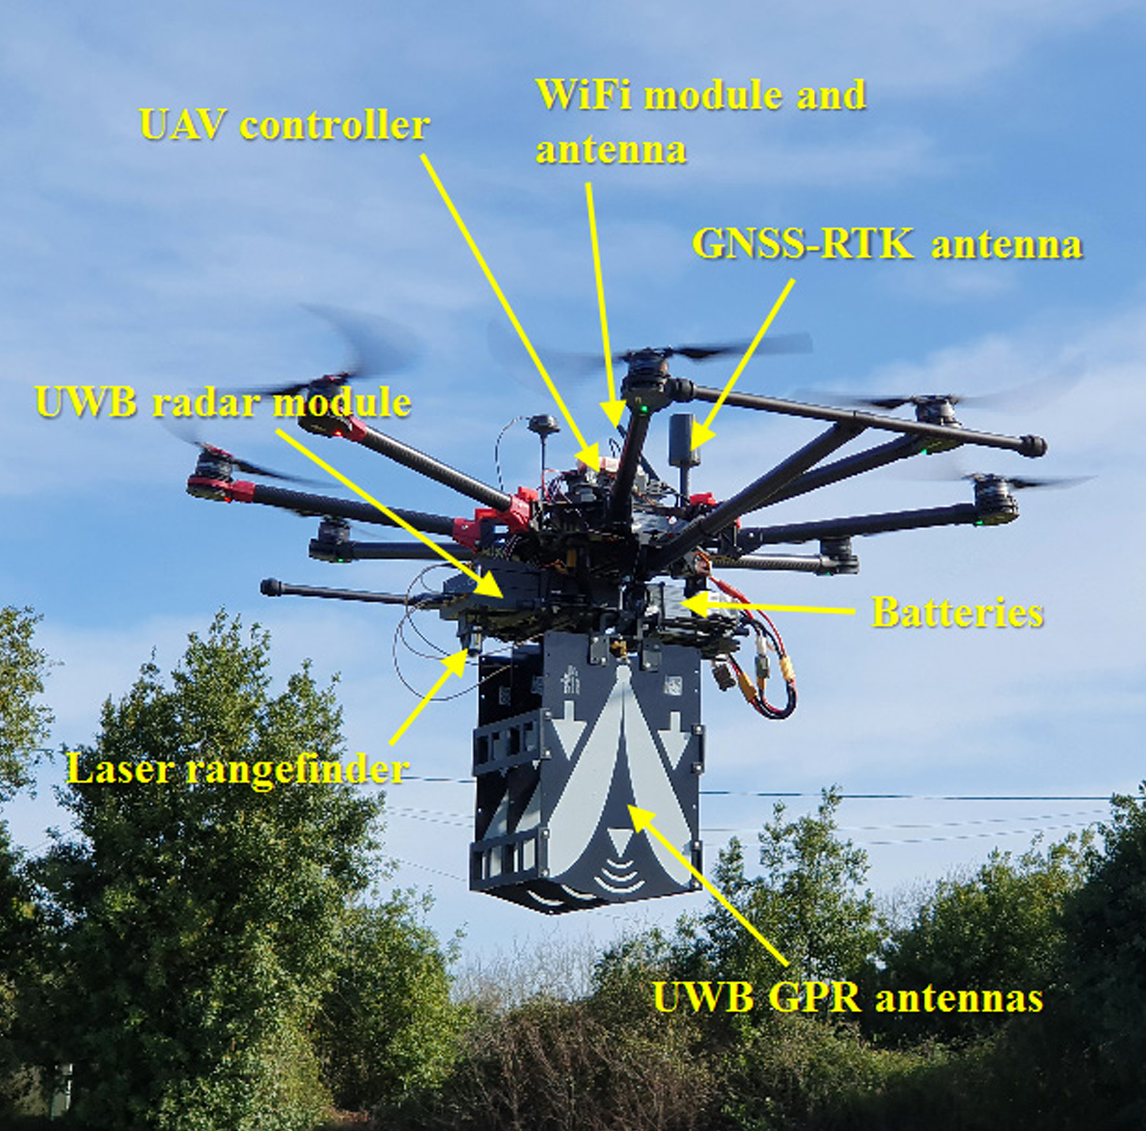
\includegraphics[height=5cm]{figs/Huirui/gpr_drone1.png}
        \label{fig:gpr_drone1}
    \end{subfigure}
    \hfill
    \begin{subfigure}[b]{0.48\linewidth}
        \centering
        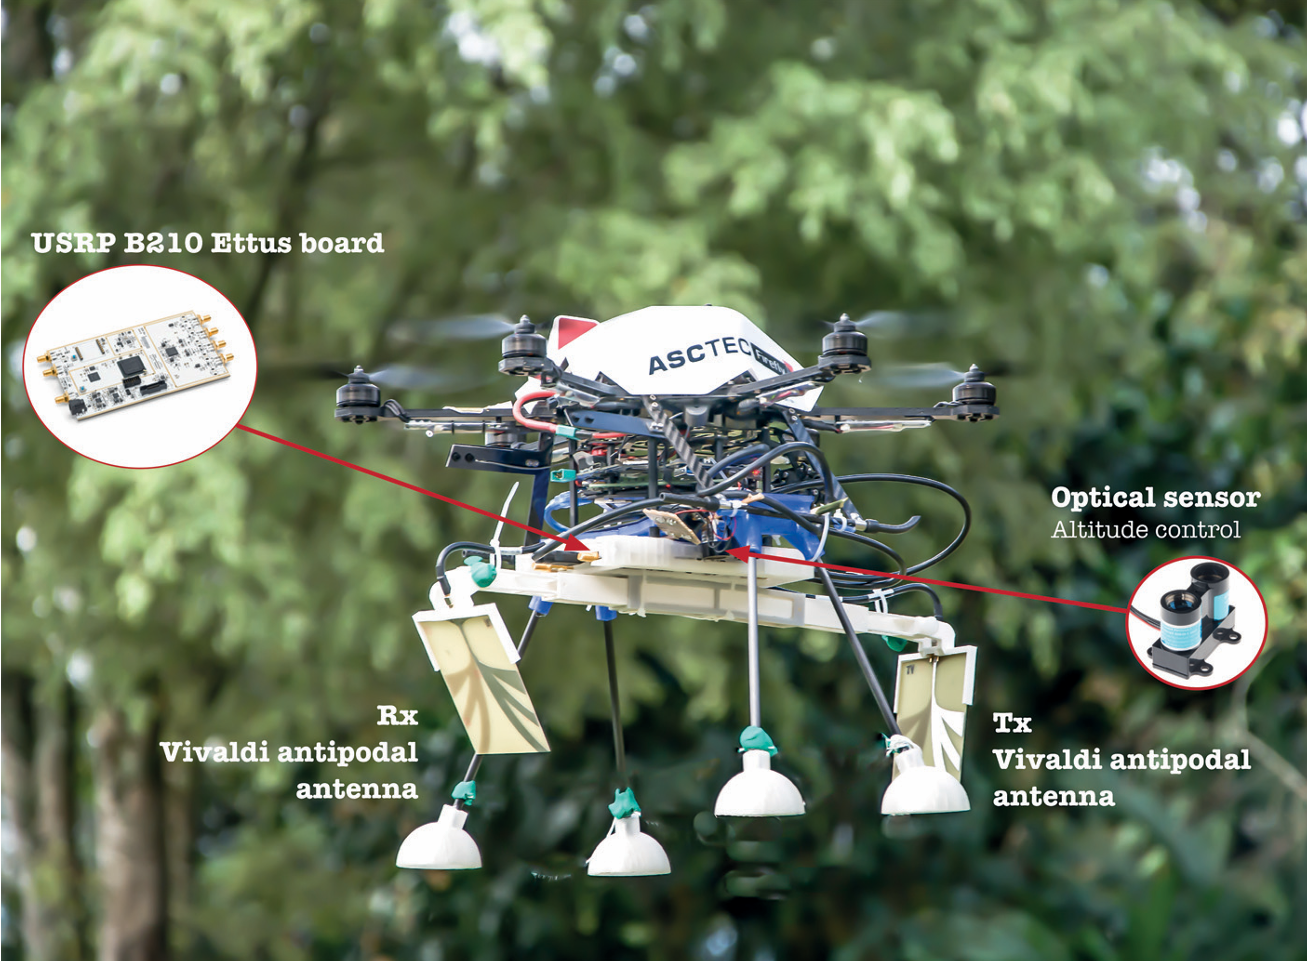
\includegraphics[height=5cm]{figs/Huirui/gpr_drone2.png}
        \label{fig:gpr_drone2}
    \end{subfigure}
    \caption{Examples of UAV platforms integrating GPR systems for landmine detection.~\cite{garcia2022safedrone,cerquera2017uav}}
    \label{fig:gpr_uav_examples}
\end{figure}

\gls{UAV}-based \gls{GPR} systems have demonstrated strong capabilities in detecting both metallic and non-metallic buried landmines~\cite{vsipovs2020lightweight,colorado2017integrated}. They are relatively robust against surface clutter and can operate under various weather and lighting conditions~\cite{noviello2022overview}. However, their effectiveness is significantly reduced in highly conductive or moist soils where radar signals experience strong attenuation in underground transmission~\cite{lee2023modeling}. Additionally, rough or cluttered terrain can interfere with signal clarity due to increased scattering and poor coupling with the ground~\cite{yoo2021application}. Signal attenuation from altitude and scattering at the air-soil interface might also obscure returns from shallow targets~\cite{garcia2019autonomous}. Despite recent progress in lightweight system development (e.g., 250 g and 5 W \gls{GPR} systems)~\cite{colorado2017integrated}, low-altitude operation (typically between 0.5--2.5 meters) remains essential for accurately detecting small or shallow landmines, which increases flight risk and limits area coverage efficiency~\cite{vsipovs2020lightweight,colorado2017integrated,fernandez2021development}.



\subsubsection{Spectral and Thermal Imaging Systems}\label{spectral_imaging}

Spectral and thermal imaging systems utilize differences in electromagnetic radiation reflected or emitted from the Earth's surface to detect surface or near-surface anomalies. These techniques are commonly used to identify thermal or visual signatures associated with landmines, disturbed soil, or stressed vegetation. The three principal sensor types in this class are optical (RGB) cameras, \gls{IR} imagers, and hyperspectral/multispectral sensors.

\textbf{Optical cameras} operate in the visible spectrum and are typically used for detecting surface-laid landmines or areas of disturbed terrain based on color, shape, or texture differences~\cite{cardonalandmine}. \textbf{Thermal infrared imaging} measures variations in surface temperature caused by differing thermal conductivities and capacities between buried mines and the surrounding soil. These differences are most detectable during transitional periods such as early morning or late evening and may stem from either volume effects or surface effects related to burial~\cite{Bruschini1997ASO,paik2002image,hutsul2024review}. \textbf{Hyperspectral and multispectral imaging} systems, which span from visible to shortwave infrared wavelengths, are capable of identifying subtle spectral anomalies in vegetation or soil that could indicate the presence of buried mines~\cite{robledo2009survey,alqudsi2021review}.

\paragraph{Drone Applications} \gls{UAV}-based spectral imaging systems have been extensively deployed in landmine detection studies~\cite{dena2020image,10.1117/12.2177182,Popov2022MethodFM,rs15040967,Baur2021HowTI,baur2020applying,AgrawalChung2024ComparingSL,10765909,6842242,rs16122046,qiu2023joint,ptsa-qj43-23,TENORIOTAMAYO2023109443,nikulin2018detection,FORERORAMIREZ2022104307,TENORIOTAMAYO2024105567,krause2018diurnal,Fardoulis2020PROOFHS,butt2024uav}. Figures~\ref{fig:thermal_camera_drone} and~\ref{fig:optical_camera_drone} illustrate \gls{UAV}s equipped with thermal and multispectral sensors, respectively, for aerial landmine detection.

\begin{figure}[h!]
    \centering
    \begin{subfigure}[b]{0.48\linewidth}
        \centering
        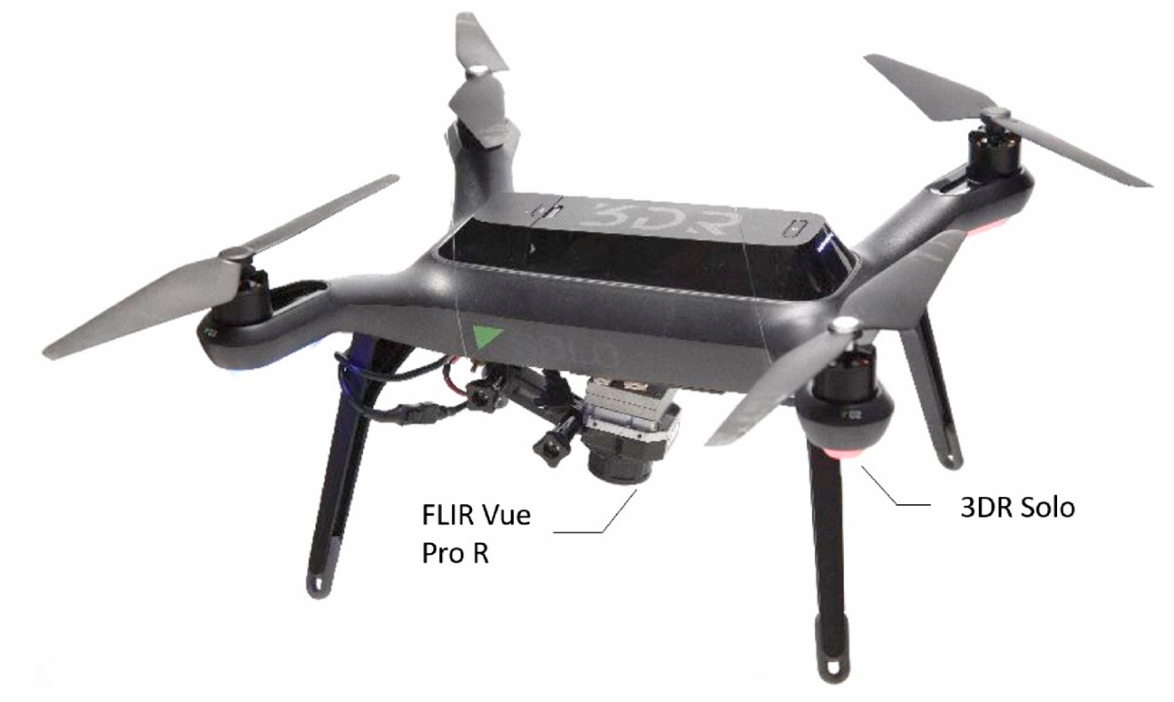
\includegraphics[height=3.5cm]{figs/Huirui/thermal_camera_drone.png}
        \caption{Thermal infrared camera mounted on UAV~\cite{nikulin2018detection}.}
        \label{fig:thermal_camera_drone}
    \end{subfigure}
    \hfill
    \begin{subfigure}[b]{0.48\linewidth}
        \centering
        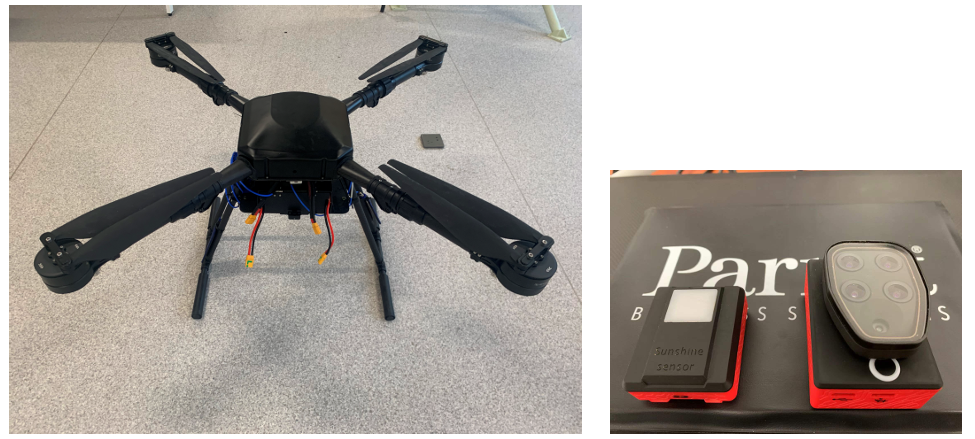
\includegraphics[height=3.5cm]{figs/Huirui/multispectral_drone.png}
        \caption{Multispectral camera mounted on UAV~\cite{qiu2023joint}.}
        \label{fig:optical_camera_drone}
    \end{subfigure}
    \caption{Examples of UAV-mounted spectral sensors used in landmine detection.}
    \label{fig:spectral_camera_drones}
\end{figure}

Among the available aerial spectral imaging approaches, thermal infrared cameras is the only one effective for detecting both surface and shallowly buried landmines. They can be deployed at altitudes of 5--10 meters while maintaining satisfactory detection accuracy~\cite{TENORIOTAMAYO2024105567,rs15040967}. Optical (RGB) cameras offer a low-cost and lightweight solution for identifying visible surface anomalies but are limited in vegetated or obscured environments and cannot detect buried landmines~\cite{Baur2021HowTI,6842242,rs16122046}. Hyperspectral and multispectral systems provide richer spectral information and can be used to detect soil or vegetation disturbances with high material specificity~\cite{10765909}. However, they are not optimized for the \gls{LWIR} range necessary for detecting subsurface objects~\cite{ptsa-qj43-23}. Furthermore, their high cost (up to twelve times greater than thermal infrared cameras) limits their practical use in large-scale \gls{UAV} demining missions~\cite{rs15040967}.



\subsubsection{Other Detection Methods}\label{other_detection_methods}

In addition to the mainstream sensing methods discussed above, several alternative techniques have been explored for landmine detection. These include mechanical, acoustic, chemical, and biological approaches. While some of these methods have demonstrated promising results in controlled or ground-based experiments, they remain largely underexplored in \gls{UAV}-based applications.

\textbf{Mechanical and vibro-acoustic} methods identify landmines by analyzing their unique vibrational or acoustic responses to external stimuli. These techniques typically involve the transmission of low-frequency acoustic or seismic waves into the ground and the measurement of reflected signals using either contact or non-contact sensors. Buried landmines can be distinguished from background materials such as rocks or roots by their characteristic resonant signatures~\cite{Gooneratne2004ARO,gichd2006guidebook}. Ultrasound-based methods follow a similar principle, using high-frequency acoustic waves (above 20 kHz) to image subsurface features based on wave reflections from material boundaries~\cite{paik2002image,cardonalandmine}. Although effective in controlled tests, these methods generally require physical coupling with the ground or close-range proximity, making them unsuitable for most \gls{UAV} platforms.

\textbf{Chemical and biological} detection methods aim to identify explosive materials through emitted vapors or chemical markers. Chemical sensors based on polymer films or photoluminescent coatings, as well as biological agents such as trained animals or genetically modified bacteria, have been developed to detect compounds like \gls{TNT}~\cite{Gooneratne2004ARO,alqudsi2021review}. One example involves the deployment of fluorescent bacteria over suspected minefields, with subsequent monitoring for a visible reaction~\cite{cardonalandmine}. However, these techniques face major challenges in drone integration, including the difficulty of sampling trace vapors from altitude and ensuring consistent sensor performance in variable environmental conditions.



\subsubsection{Comparative Summary and Method Selection}\label{sensor_compare_select}

The goal of this project is to develop a \gls{UAV}-based landmine detection system capable of identifying both surface-laid and buried anti-personnel landmines. To ensure operational safety and efficient area coverage, the selected sensors must be suitable for aerial deployment at altitudes above 1 meter and must be rigidly mounted on the drone platform. In this context, three classes of sensing approaches are considered: \textbf{magnetometers}, \textbf{\gls{GPR}}, and \textbf{spectral imaging sensors}, including optical, thermal, and hyperspectral or multispectral cameras. The quantitative comparison of the evaluated sensors (1 = very favorable, 5 = very unfavorable) on detection capability, accuracy, power usage, system complexity, and cost, with is summarized in Table~\ref{tab:sensor_comparison}.


\begin{table}[h]
    \centering
    \small
    \renewcommand{\arraystretch}{1.3}
    \caption{Quantitative comparison of UAV-compatible landmine detection.}
    \label{tab:sensor_comparison}
    \begin{tabular}{l c c c c c c c}
        \toprule
        \textbf{Sensor Type} & \textbf{Robustness} & \textbf{Accuracy} & \textbf{Power} & \textbf{Weight} & \textbf{Complexity} & \textbf{Cost} & \textbf{Total} \\
        \midrule
        Thermal \gls{IR} Camera        & 2 & 2 & 2 & 2 & 2 & 2 & 12 \\
        Ground Penetrating Radar & 1 & 1 & 3 & 3 & 3 & 3 & 14 \\
        Magnetometer             & 5 & 3 & 1 & 2 & 3 & 1 & 15 \\
        Optical Camera           & 5 & 4 & 1 & 1 & 1 & 1 & 13 \\
        Hyperspectral Sensor     & 4 & 3 & 5 & 5 & 5 & 5 & 27 \\
        \bottomrule
    \end{tabular}
\end{table}

From Table~\ref{tab:sensor_comparison}, most options except hyperspectral cameras receive similar overall scores. This suggests that no single technique can offer both wide-area coverage and accurate detection. Since these sensors can be broadly divided into \textbf{high-altitude} imaging systems (thermal or optical cameras) and \textbf{low-altitude} subsurface sensors (magnetometers or \gls{GPR}), to ensure both efficiency and accuracy, a \textbf{layered sensing strategy} in which a high-altitude scan identifying regions of interest is followed by low-altitude inspections over those areas is adopted.

For high-altitude scanning, \textbf{thermal infrared imaging} is preferred over optical camera because the later one is limited to detecting visible surface features and cannot identify buried landmines. For low-altitude validation, \textbf{\gls{GPR}} is selected over magnetometers due to its ability to detect both metallic and non-metallic landmines and a possible safer flight altitude (above 1 m).

The final system design therefore integrates a thermal infrared camera for high-altitude scanning and a \gls{GPR} for low-altitude confirmation. Details of the sensors' working principles and system configurations are presented in the following sections. 

The final system design therefore integrates a thermal infrared camera for high-altitude scanning and a \gls{GPR} for low-altitude confirmation. Compared with alternative configurations, this sequential architecture has been shown to significantly improve time efficiency~\ref{sec:msp_comparison_manual_demining}, with only a minor reduction in overall detection performance~\ref{fusion_bounds}. Details of the sensors’ working principles and system configurations are presented in the following sections.